\section*{ÔN TẬP KIỂM TRA CUỐI KÌ 1 - ĐỀ 04}
\setcounter{ex}{0}\setcounter{bt}{0}
\Opensolutionfile{ans}[ans/ansBTTeX4]

\begin{ex}%[Đoàn Minh Tân]%[0D4Y5-1]
Bảng xét dấu nào dưới đây là của tam thức $f(x)=-x^2+6x-9$?
\choice
{
\begin{tikzpicture}
\tkzTabInit[nocadre=false, lgt=1.5, espcl=1.5]
{$x$ /0.6,$f(x)$ /0.6}
{$-\infty$,$3$, $+\infty$}
\tkzTabLine{,+,0,-}
\end{tikzpicture}
}
{
\begin{tikzpicture}
\tkzTabInit[nocadre=false, lgt=1.5, espcl=1.5]
{$x$ /0.6,$f(x)$ /0.6}
{$-\infty$,$3$, $+\infty$}
\tkzTabLine{,-,0,+}
\end{tikzpicture}
}
{\True 
\begin{tikzpicture}
\tkzTabInit[nocadre=false, lgt=1.5, espcl=1.5]
{$x$ /0.6,$f(x)$ /0.6}
{$-\infty$,$3$, $+\infty$}
\tkzTabLine{,-,0,-}
\end{tikzpicture}
}
{
\begin{tikzpicture}
\tkzTabInit[nocadre=false, lgt=1.5, espcl=1.5]
{$x$ /0.6,$f(x)$ /0.6}
{$-\infty$,$3$, $+\infty$}
\tkzTabLine{,+,0,+}
\end{tikzpicture}
}
\loigiai{
Tam thức $f(x)=-x^2+6x-9$ có $\Delta=0$, nghiệm kép $x=3$ và hệ số $a=-1<0$ nên có bảng xét dấu như sau
\begin{center}

\begin{tikzpicture}
\tkzTabInit[nocadre=false, lgt=1.5, espcl=1.5]
{$x$ /0.6,$f(x)$ /0.6}
{$-\infty$,$3$, $+\infty$}
\tkzTabLine{,-,0,-}
\end{tikzpicture}
\end{center}
}
\end{ex}

\begin{ex}%[Đoàn Minh Tân]%[0D4Y5-1]
Bảng xét dấu nào sau đây là bảng xét dấu của tam thức $f(x)=-x^2-x+6$?
\choice
{
\begin{tikzpicture}
\tkzTabInit[nocadre=false, lgt=1.5, espcl=1.5]
{$x$ /0.6,$f(x)$ /0.6}
{$-\infty$,$-2$,$3$, $+\infty$}
\tkzTabLine{,-,0,+,0,-}
\end{tikzpicture}
}
{
\begin{tikzpicture}
\tkzTabInit[nocadre=false, lgt=1.5, espcl=1.5]
{$x$ /0.6,$f(x)$ /0.6}
{$-\infty$,$-2$,$3$, $+\infty$}
\tkzTabLine{,+,0,-,0,+}
\end{tikzpicture}
}
{\True 
\begin{tikzpicture}
\tkzTabInit[nocadre=false, lgt=1.5, espcl=1.5]
{$x$ /0.6,$f(x)$ /0.6}
{$-\infty$,$-3$,$2$, $+\infty$}
\tkzTabLine{,-,0,+,0,-}
\end{tikzpicture}
}
{
\begin{tikzpicture}
\tkzTabInit[nocadre=false, lgt=1.5, espcl=1.5]
{$x$ /0.6,$f(x)$ /0.6}
{$-\infty$,$-3$,$2$, $+\infty$}
\tkzTabLine{,+,0,-,0,+}
\end{tikzpicture}
}
\loigiai{
Tam thức $f(x)=-x^2-x-6$ có $\Delta =25>0$, hai nghiệm $x_1=-3$, $x_2=2$ và hệ số $a=-1<0$.\\
Suy ra bảng xét dấu của $f(x)$ như sau
\begin{center}

\begin{tikzpicture}
\tkzTabInit[nocadre=false, lgt=1.5, espcl=1.5]
{$x$ /0.6,$f(x)$ /0.6}
{$-\infty$,$-3$,$2$, $+\infty$}
\tkzTabLine{,-,0,+,0,-}
\end{tikzpicture}
\end{center}
}
\end{ex}

\begin{ex}%[Trần Quốc, BG10-2022, Nhóm 9]%[0H1Y3-1]
\immini{Cho đoạn thẳng $AB$ và điểm $I$ thuộc đoạn thẳng $AB$ như hình vẽ bên. Mệnh đề nào sau đây đúng?
\choice
{$\overrightarrow{AI}=\dfrac{1}{4}\overrightarrow{AB}$}
{\True $\overrightarrow{AI}=\dfrac{1}{4}\overrightarrow{IB}$}
{$\overrightarrow{AI}=\dfrac{1}{5}\overrightarrow{BA}$}
{$\overrightarrow{AI}=-\dfrac{1}{4}\overrightarrow{IB}$}}
{    \begin{tikzpicture}[scale=1,font=\footnotesize,line join = round, line cap = round, >= stealth]
\clip (-1,-1) rectangle (6,1);
\tkzDefPoints{0/0/A, 5/0/B, 1/0/I}
\draw (A)--(B);
\foreach \x in {A,B,I} \fill (\x) circle(1pt) node[{shift=(90:0.25)}]{$\x$};
\foreach \x in {2,3,4} \fill (\x,0) circle(1pt);
\end{tikzpicture}}
\loigiai{
Từ hình vẽ ta có $\overrightarrow{AI}=\dfrac{1}{4}\overrightarrow{IB}$.
}
\end{ex}

\begin{ex}%[Lê Minh Thiện Anh, Dự án BG10-Lần2]%[0H1Y1-3]
Cho hình bình hành $ABCD$, mệnh đề nào trong các mệnh đề sau đây là \textbf{đúng}?
\choice
{\True $\overrightarrow{AB}=\overrightarrow{DC}$}
{$\overrightarrow{AD}=\overrightarrow{CB}$}
{$\overrightarrow{CA}=\overrightarrow{DB}$}
{$\overrightarrow{AB}=\overrightarrow{CD}$}
\loigiai
{Do $ABCD$ là hình bình hành nên $\overrightarrow{AB}=\overrightarrow{DC}$.
\begin{center}
\begin{tikzpicture}[scale=1, font=\footnotesize,line join=round, line cap=round, >=stealth]
\coordinate (A) at (0,0);
\coordinate (B) at (3,0);
\coordinate (D) at (-1.5,-1);
\coordinate (C) at ($(D)+(B)-(A)$);
\tkzDrawPoints[fill=black](A,B,C,D)
\draw (A)node[above]{$A$} -- (B)node[above]{$B$};
\draw (C)node[below]{$C$} -- (D)node[below]{$D$} (B)--(C);
\draw (A)--(C) (A)--(D) (B)--(D);
\end{tikzpicture}
\end{center}}
\end{ex}

\begin{ex}%[0D2Y3-1]%[Trần Ngọc Phú - Dự án TLDH5]
\immini{Tìm hàm số bậc hai có bảng biến thiên như hình vẽ bên.
\choice
{\True $y=x^2-4x+5$}
{$y=x^2-2x+1$}
{$y=-x^2+4x-3$}
{$y=x^2-4x-5$}}
{
\begin{tikzpicture}
\tkzTabInit[nocadre=false,lgt=1,espcl=2.5,deltacl=0.6]
{$x$ /0.6, $y$ /1.5}
{$-\infty$,$2$,$+\infty$}
\tkzTabVar{+/$+\infty$,-/$1$,+/$+\infty$}
\end{tikzpicture}
}
\loigiai{
Dựa vào bảng biến thiên ta có $a > 0$ và hàm số có tọa độ đỉnh là $(2;1)$.\\Vậy hàm số $y=x^2-4x+5$ thỏa bảng biên thiên.
}
\end{ex}

\begin{ex}%[0D4Y4-1]
Điểm $A(-1;3)$ thuộc miền của bất phương trình
\choice
{$x+3y<0$}
{$3x-y>0$}
{\True  $-3x+2y-4>0$}
{$2x-y+4>0$}
\loigiai{
Thay tọa độ $A(-1;3)$ vào các bất phương trình:
\begin{itemize}
\item[•] Với bất phương trình $x+3y<0$, ta có $(-1)+3\cdot 3<0$ sai.
\item[•] Với bất phương trình $3x-y>0$, ta có $3\cdot (-1)-3>0$ sai.
\item[•] Với bất phương trình $-3x+2y-4>0$, ta có $-3\cdot (-1)+2\cdot 3-4>0$ đúng.
\item[•] Với bất phương trình $2x-y+4>0$, ta có $2\cdot (-1)-3+4>0$ sai.
\end{itemize}
Vậy $A(-1;3)$ thuộc miền nghiệm bất phương trình $-3x+2y-4>0$.
}
\end{ex}

\begin{ex}%[Phan Quốc Trí, Bai Giảng T10(2022)]%[0D1Y1-3]
Cho mệnh đề $P\colon$ \lq\lq  $9$ là số chia hết cho $3$\rq\rq. Mệnh đề phủ định của mệnh đề $P$ là
\choice
{$\overline{P}\colon$\lq\lq  $9$ là ước của $3$\rq\rq}
{$\overline{P}\colon$\lq\lq  $9$ là bội của $3$\rq\rq}
{\True $\overline{P}\colon$ \lq\lq  $9$ là số không chia hết cho $3$\rq\rq}
{$\overline{P}\colon$\lq\lq  $9$ là số lớn hơn $3$\rq\rq}
\loigiai{Mệnh đề $P\colon$\lq\lq  $9$ là số chia hết cho $3$\rq\rq      có mệnh đề phủ định là $\overline{P}\colon$ \lq\lq  $9$ là số không chia hết cho $3$\rq\rq.}
\end{ex}

\begin{ex}%[Trần Minh,Chuyển sách Tex - 10, 11 (dự án 3)]%[0H2Y3-1]
Tam giác $ ABC$ có $ AB=5$, $BC=7$, $CA=8$. Số đo góc $ \widehat{A}$ bằng
\choice
{$ 30^\circ $}
{$ 45^\circ $}
{\True $ 60^\circ $}
{$ 90^\circ $}
\loigiai
{Theo định lí hàm cô-sin, ta có $ \cos{A}=\dfrac{AB^2+AC^2-BC^2}{2AB\cdot AC}=\dfrac{5^2+8^2-7^2}{2\cdot 5\cdot 8}=\dfrac{1}{2}$.\\
Do đó, $ \widehat{A}=60^\circ $.}
\end{ex}

\begin{ex}%[0H2Y2-1]
Cho hình vuông $ABCD$ cạnh $a$. Tính tích vô hướng của hai véc-tơ $\overrightarrow{AB}$ và $\overrightarrow{AC}$.
\choice
{$\overrightarrow{AB}\cdot\overrightarrow{AC}=a\sqrt{2}$}
{$\overrightarrow{AB}\cdot\overrightarrow{AC}=2a$}
{\True $\overrightarrow{AB}\cdot\overrightarrow{AC}=a^2$}
{$\overrightarrow{AB}\cdot\overrightarrow{AC}=2a^2$}
\loigiai{
Ta có $\overrightarrow{AB}\cdot\overrightarrow{AC}=|\overrightarrow{AB}|\cdot|\overrightarrow{AC}|\cdot\cos(\overrightarrow{AB},\overrightarrow{AC})=a\cdot a\sqrt{2}\cos 45^\circ=a^2$.
}
\end{ex}

\begin{ex}%[0H2Y3-1]
Tam giác $ ABC$ có $ AB=\sqrt{2}$, $AC=\sqrt{3}$ và $ \widehat{C}=45^\circ $. Tính độ dài cạnh $ BC$.
\choice
{$ BC=\sqrt{5}$}
{\True $ BC=\dfrac{\sqrt{6}+\sqrt{2}}{2}$}
{$ BC=\sqrt{6}$}
{$ BC=\dfrac{\sqrt{6}-\sqrt{2}}{2}$}
\loigiai
{Theo định lí hàm cosine, ta có\\
$ AB^2=AC^2+BC^2-2\cdot AC\cdot BC\cdot \cos \widehat{C}\Rightarrow {(\sqrt{2} )}^2={(\sqrt{3} )}^2+BC^2-2\cdot \sqrt{3}\cdot BC\cdot \cos 45^\circ $ \\
$ \Rightarrow BC=\dfrac{\sqrt{6}+\sqrt{2}}{2}$.}
\end{ex}

\begin{ex}%[0D4Y4-4]
Miền nghiệm của hệ bất phương trình $\heva{& x-y\ge 3 \\ & 2x+y<4}$ chứa điểm nào trong các điểm sau?
\choice
{\True $(1;-3)$}
{$(-2;1)$}
{$(3;-2)$}
{$(4;1)$}
\loigiai{Thay điểm $(1;-3)$ vào hệ bất phương trình, ta có
$\heva{& 1-(-3) = 4 \ge 3 \\ & 2 \cdot 1 + (-3) = -2 <4}$ (đúng).
}
\end{ex}

\begin{ex}%[0D2Y3-3]
Trục đối xứng của parabol $y=-x^2+5x+3$ là đường thẳng có phương trình
\choice
{$x=\dfrac{5}{4}$}
{$x=-\dfrac{5}{2}$}
{$x=-\dfrac{5}{4}$}
{\True $x=\dfrac{5}{2}$}
\loigiai{
Trục đối xứng của parabol $y=a{x^2}+bx+c$ là đường thẳng $x=-\dfrac{b}{2a}$ .\\
Trục đối xứng của parabol $y=-x^2+5x+3$ là đường thẳng $x=\dfrac{5}{2}$.}
\end{ex}

\begin{ex}%[Phan Quốc Trí, Bai Giảng T10(2022)]%[0D1Y2-2]
Có bao nhiêu tập $ X $ thỏa mãn $ \{a;b\} \subset X \subset \{1;2;a;b\}$?
\choice
{$3$}
{$2$}
{\True $4$}
{$5$}
\loigiai{
Các tập $ X $ thỏa mãn là $ \{a;b\} $, $ \{1;a;b\} $, $ \{2;a;b\} $, $ \{1;2;a;b\} $.
}
\end{ex}


\begin{ex}%[0H2B1-1]
Khẳng định nào sau đây đúng?
\choice
{$\sin 90^\circ <\sin 150^\circ $}
{$\sin 90^\circ 1{5}'<\sin 90^\circ 30'$}
{\True $\cos 90^\circ 30'>\cos 100^\circ $}
{$\cos 150^\circ >\cos 120^\circ $}
\loigiai
{Trong khoảng từ $90^\circ $ đến $180^\circ $, khi giá trị của góc tăng thì:\\
- Giá trị $\sin$ tương ứng của góc đó giảm.\\
- Giá trị $\cos$ tương ứng của góc đó giảm.}
\end{ex}

\begin{ex}%[0D6BH-2]%[0D3B2-4]
Nghiệm của phương trình $\sqrt{x^2 - 2x + 4} = \sqrt{2 - x}$ là
\choice
{$x = \dfrac{1}{2} $}
{$x = \dfrac{7}{4} $}
{$\hoac{& x = \frac{1}{2} \\& x = \dfrac{7}{4}}$}
{\True $x \in \varnothing $}
\loigiai{
Điều kiện: $\heva{&x^2 - 2x + 4 \geq 0\\&2 - x \geq 0} \Leftrightarrow \heva{&x  \in \mathbb{R}\\&x \leq 2} \Leftrightarrow x \leq 2$.\\
Ta có
\allowdisplaybreaks
\begin{eqnarray*}
\sqrt{x^2 - 2x + 4} = \sqrt{2 - x}
&\Leftrightarrow&x^2 - 2x + 4 = 2 - x\\
&\Leftrightarrow&x^2 - x + 2 =  0 \;\;\text{(vô nghiệm)}
\end{eqnarray*}
Vậy phương trình đã cho vô nghiệm.
}
\end{ex}

\begin{ex}%[0H2B2-1]
Cho $\triangle ABC$ đều cạnh bằng $3$. Trên các cạnh $AB, AC$ lần lượt lấy các điểm $M,N$ sao cho $2AM=MB, NA=2NC$. Giá trị của tích vô hướng $\overrightarrow{BN}\cdot \overrightarrow{CM}$ là
\choice
{$\dfrac{7}{2}$}
{\True $-\dfrac{7}{2}$}
{$\dfrac{11}{2}$}
{$-\dfrac{11}{2}$}
\loigiai{
\immini{
\begin{eqnarray*}
\overrightarrow{BN}\cdot \overrightarrow{CM}&=&\left( \overrightarrow{AN}-\overrightarrow{AB} \right) \cdot \left( \overrightarrow{AM}-\overrightarrow{AC} \right)\\
&=&\overrightarrow{AN}\cdot \overrightarrow{AM}-\overrightarrow{AN}\cdot\overrightarrow{AC}-\overrightarrow{AB}\cdot\overrightarrow{AM}+\overrightarrow{AB}\cdot\overrightarrow{AC}\\
&=&1\cdot 2 \cdot \cos 60^{\circ} -2 \cdot 3 \cos 0^{\circ} -3 \cdot 1 \cos 0^{\circ} +3 \cdot 3 \cos 60^{\circ}\\
&=&-\dfrac{7}{2}.
\end{eqnarray*}
}{
\begin{tikzpicture}[scale=0.8, font=\footnotesize, line join=round, line cap=round, >=stealth]
\tkzDefPoints{0/0/B, 6/0/C, 3/3/A}
\tkzDefPointBy[homothety=center A ratio 0.33 ](B) \tkzGetPoint{M}
\tkzDefPointBy[homothety=center A ratio 0.66 ](C) \tkzGetPoint{N}
\tkzDrawSegments(A,B B,C C,A C,M B,N)
\tkzDrawPoints(B,C,A,M,N)
\tkzLabelPoints[below](B,C)
\tkzLabelPoints[above](A)
\tkzLabelPoints[left](M)
\tkzLabelPoints[right](N)
\end{tikzpicture}
}
}
\end{ex}

\begin{ex}%[0D3B2-4]
Nghiệm của phương trình $\sqrt{x-1}=\left(\sqrt{3-x}\right)^2$ là
\choice
{$x=2;x=5$}
{\True $x=2$}
{$x=1;x=3$}
{$x=-1;x=-3$}
\loigiai{
Ta có
\allowdisplaybreaks
\begin{eqnarray*}
\sqrt{x-1}=\left(\sqrt{3-x}\right)^2	&\Rightarrow & \sqrt{x-1}=3-x\\
& \Rightarrow  & x-1=(3-x)^2 \\
& \Rightarrow & x^2-7x+10=0\\
&\Rightarrow & \hoac{&x=2\\&x=5}.
\end{eqnarray*}
Chỉ có nghiệm $x=2$ thỏa mãn phương trình ban đầu. \\
Vậy $S=\{2\}$.
}
\end{ex}

\begin{ex}%[Huỳnh Đức Vũ, BG10-2022, Nhóm 9]%[0H1B3-2]
Cho tam giác $ABC$ biết $I$ là trung điểm của đoạn thẳng $AB$, $G$ là trọng tâm tam giác, $M$ là điểm bất kỳ. Hãy chọn khẳng định \textbf{đúng}.
\choice
{$\overrightarrow{MA}+\overrightarrow{MB}+\overrightarrow{MC}=2\overrightarrow{MG}$}
{$\overrightarrow{BI}+\overrightarrow{IC}=\overrightarrow{0}$}
{$\overrightarrow{MA}+\overrightarrow{MB}=3\overrightarrow{MI}$}
{\True $\overrightarrow{MA}+\overrightarrow{MB}+\overrightarrow{MC}=3\overrightarrow{MG}$}
\loigiai
{\begin{itemize}
\item Vì $\overrightarrow{BI}+\overrightarrow{IC}=\overrightarrow{BC}$ nên phương án $\overrightarrow{BI}+\overrightarrow{IC}=\overrightarrow{0}$ là phương án \textbf{sai}.
\item Vì $\overrightarrow{MA}+\overrightarrow{MB}=2\overrightarrow{MI}$ nên phương án $\overrightarrow{MA}+\overrightarrow{MB}=3\overrightarrow{MI}$ là phương án \textbf{sai}.
\item Theo quy tắc trọng tâm tam giác ta có $ \overrightarrow{MA}+\overrightarrow{MB}+\overrightarrow{MC} = 3\overrightarrow{MG}$.
\end{itemize} }
\end{ex}

\begin{ex}%[0D2B1-3]
\immini{
Cho hàm số $y=f(x)$ có tập xác định là $[-3;3]$ và đồ thị của nó được biểu diễn bởi hình bên. Khẳng định nào dưới đây là đúng?
\choice
{Hàm số nghịch biến trên khoảng $(1;0)$}
{Hàm số nghịch biến trên khoảng $(0;3)$}
{\True Hàm số nghịch biến trên khoảng $(-1;1)$}
{Hàm số đồng biến trên khoảng $(-1;4)$}
}{
\begin{tikzpicture}
\draw[>=stealth,->] (-2.5,0) -- (3.5,0) node[above]{\scriptsize $x$};
\draw[>=stealth,->] (0,-1.5) -- (0,2.5) node[left]{\scriptsize $y$};
\draw (0,0) node[below left]{\scriptsize $O$};
\draw [thick] (-2,0)--(-1,1)--(1,-1)--(3,2);
\foreach \i in {-2,-1,1,3}
\draw (\i,0.03) -- (\i,-0.03);
\foreach \i in {-1,1,2}
\draw (0.03,\i) -- (-0.03,\i);
\foreach \i in {-2,-1,1,3}
\draw (\i,0) node[below]{\scriptsize $\i$};
\foreach \i in {-1,1,2}
\draw (0,\i) node[right]{\scriptsize $\i$};
\draw [dashed] (-1,0)|-(-1,1) (1,0)|-(0,-1);
\draw [dashed] (3,0)|-(0,2);
\end{tikzpicture}
}
\loigiai{Dựa vào đồ thị hàm số, ta có hàm số nghịch biến trên khoảng $(-1;1)$.}
\end{ex}

\begin{ex}%[Đỗ Đường Hiếu - ĐCHT THPT]%[0D1B3-2]
\immini{Cho các tập hợp $ A$, $ B$, $ C$ được minh họa bằng biểu đồ Ven như hình bên. Phần tô màu xám trong hình là biểu diễn của tập hợp nào sau đây?\\
\choice
{$ A\cap B\cap C$}
{$\left(A\setminus C\right)\cup\left(A\setminus B\right)$}
{$\left(A\cup B\right)\setminus C$}
{\True $\left(A\cap B\right)\setminus C$}}
{\begin{tikzpicture}[scale=1, line join=round, line cap=round]
\coordinate (A) at (0,0);
\coordinate (B) at (2,0);
\coordinate (C) at (1,-1.5);
\begin{scope}
\clip (A) circle (1.5);
\fill[pattern=north west lines] (B) circle (1.5);
\end{scope}
\fill[white] (C) circle (1.5);
\draw (A) circle (1.5);
\draw (B) circle (1.5);
\draw (C) circle (1.5);
\path
(A)++(90:.6) node[fill=white,above]{$A$}
(B)++(90:.6) node[fill=white,above]{$B$}
(C)++(-90:1) node[fill=white,above]{$C$};
\end{tikzpicture}}
\loigiai{
Sử dụng phép toán giao hai tập hợp để tìm $ A\cap B$, từ đó suy ra phần tô màu xám trong hình là biểu diễn của tập hợp $\left(A\cap B\right)\setminus C$.
}
\end{ex}

\begin{ex}%[0D2B3-1]%[Trần Ngọc Phú - Dự án TLDH5]
Hàm số nào sau đây có giá trị lớn nhất bằng $5$?
\choice
{$y=x^2-4x-8$}
{$y=-x^2-2x+3$}
{$y=x^2-4x+4$}
{\True $y=-x^2-2x+4$}
\loigiai{
Để tìm giá trị lớn nhất thì điều kiện là $a>0$.\\
Ta có $y=-x^2-2x+4=-\left(x+1\right)^2+5\le 5$.\\
Vậy hàm số $y=-x^2-2x+4$ đạt giá trị lớn nhất bằng $5$ tại $x=-1$.}
\end{ex}

\begin{ex}C%[0D3B2-4]
Nghiệm của phương trình $\sqrt{4x^2+2x+10}=3x+1$ là
\choice
{\True $x=1$}
{ $x=\dfrac{-9}{5}$}
{$\hoac{&x=\dfrac{-9}{5}\\&x=1}$}
{$x\in\varnothing$}
\loigiai{Bình phương hai vế của phương trình đã cho, ta được
\begin{eqnarray*}
4x^2+2x+10=(3x+1)^2\Rightarrow 4x^2+2x+10=9x^2+6x+1\Rightarrow -5x^2-4x+9=0\Rightarrow x=1 \ \text{hoặc} \ x=-\dfrac{9}{5}.
\end{eqnarray*}
Thay lần lượt các giá trị trên vào phương trình đã cho, ta thấy $x=1$ thỏa mãn.\\
Vậy nghiệm của phương trình đã cho là $x=1$.
}
\end{ex}

\begin{ex}%[0D4B5-2]
Tập nghiệm của bất phương trình $x^2 - 5x + 6 \leq 0$ là
\choice
{$(- \infty ; 2)$}
{$( - \infty ; 2 ] \cup [3; + \infty )$}
{$[3; + \infty )$}
{\True $[2;3]$}
\loigiai{
\[x^2 - 5x + 6 = 0 \Leftrightarrow \hoac{x &=2 \\ x &=3.}\]
Bảng xét dấu
\begin{center}

\begin{tikzpicture}
\tkzTabInit[nocadre=false, lgt=2, espcl=2.5]{$x$ /1,$f(x)$ /1}{$-\infty$,$2$,$3$,$+\infty$}
\tkzTabLine{,+,$0$,-,$0$,+,}
\end{tikzpicture}
\end{center}
}
\end{ex}

\begin{ex}%[Trần Minh,Chuyển sách Tex - 10, 11 (dự án 3)]%[0H1B2-4]
Cho ba điểm phân biệt $A$, $ B$, $ C$. Mệnh đề nào sau đây đúng?
\choice
{$AB+BC=AC$}
{\True $\overrightarrow{AB}+\overrightarrow{BC}+\overrightarrow{CA}=\overrightarrow{0}$}
{$\overrightarrow{AB}=\overrightarrow{BC}\Leftrightarrow \left| \overrightarrow{CA}\right|=\left| \overrightarrow{BC}\right|$}
{$\overrightarrow{AB}-\overrightarrow{CA}=\overrightarrow{BC}$}
\loigiai{
$\overrightarrow{AB}+\overrightarrow{BC}+\overrightarrow{CA}=\overrightarrow{0}$ đúng theo quy tắc ba điểm. }
\end{ex}

\begin{ex}%[Phan Anh]%[0D2B1-1]
Điểm nào sau đây \textbf{không} thuộc đồ thị hàm số $y=\dfrac{\sqrt{x^2-4x+4}}{x}$?
\choice
{$A\left(2;0\right)$}
{$B\left(3;\dfrac{1}{3}\right)$}
{\True $C\left(1;-1\right)$}
{$D\left(-1;-3\right)$}
\loigiai{Thay từng đáp án vào hàm số $y=\dfrac{\sqrt{x^2-4x+4}}{x}$.
\begin{itemize}
\item Với $x=2$ và $y=0$, ta được $0=\dfrac{\sqrt{2^2-4.2+4}}{2}$ (đúng).
\item Với $x=3$ và $y=\dfrac{1}{3}$, ta được $\dfrac{1}{3}=\dfrac{\sqrt{3^2-4\cdot3+4}}{3}$ (đúng).
\item Với thay $x=1$ và $y=-1$, ta được $-1=\dfrac{\sqrt{1^2-4\cdot1+4}}{1}\Leftrightarrow-1=1$ (sai).
\end{itemize}}
\end{ex}

\begin{ex}%[Phan Anh]%[0D2B1-2]
Tìm tập xác định $\mathscr{D}$ của hàm số $y=\sqrt{x^2-2x+1}+\sqrt{x-3}$.
\choice
{$\mathscr{D}=(-\infty;3]$}
{$\mathscr{D}=[1;3]$}
{\True $\mathscr{D}=[3;+\infty)$}
{$\mathscr{D}=(3;+\infty)$}
\loigiai{
Hàm số xác định khi $\heva{
& x^2-2x+1\ge 0 \\
& x-3\ge 0}\Leftrightarrow \heva{
& {\left(x-1\right)}^2\ge 0 \\
& x-3\ge 0}\Leftrightarrow \heva{
& x\in \mathbb{R} \\
& x\ge 3}\Leftrightarrow x\ge 3$.\\
Vậy tập xác định của hàm số là $\mathscr{D}=\left[3;+\infty \right)$.}
\end{ex}

\begin{ex}%[Lê Minh Thiện Anh, Dự án BG10-Lần2]%[0H1B1-1]
Cho tam giác $MNP$, có thể xác định được tối đa bao nhiêu véc-tơ khác $\overrightarrow{0}$ có điểm đầu và điểm cuối là các đỉnh $M$, $N$, $P$?
\choice
{$3$}
{$27$}
{\True $6$}
{$9$}
\loigiai{
Với hai điểm phân biệt $A$ và $B$ ta sẽ có hai vectơ khác $\overrightarrow{0}$ đó là $\overrightarrow{AB}$ và $\overrightarrow{BA}$.\\
Vậy với $3$ điểm $M$, $N$, $P$ có tất cả $6$ véc-tơ thỏa mãn.
}
\end{ex}

\begin{ex}%[Trần Quốc, BG10-2022, Nhóm 9]%[0H1B3-1]
Gọi $G$ là trọng tâm tam giác vuông $ABC$ với cạnh huyền $BC=12$. vectơ $\overrightarrow{GB}-\overrightarrow{CG}$ có độ dài bằng bao nhiêu?
\choice
{\True $4$}
{$2\sqrt{3}$}
{$8$}
{$2$}
\loigiai{
\immini
{
Gọi $M$ là trung điểm của $BC$. \\
Ta có $\overrightarrow{GB}-\overrightarrow{CG}=\overrightarrow{GB}+\overrightarrow{GC}=2\overrightarrow{GM}$.\\
Vì $\triangle ABC$ vuông tại $A$ nên $AM=\dfrac{BC}{2}=6\Rightarrow GM=\dfrac{1}{3}AM=2$.\\
Vậy $\left|\overrightarrow{GB}-\overrightarrow{CG}\right|=2\left|\overrightarrow{GM}\right|=2GM=4$.
}
{
\begin{tikzpicture}[font=\footnotesize,line join=round, line cap=round, >=stealth,scale=0.8]
\tkzDefPoints{-1/0/A, -2/-2/B, 2/-2/C};
\coordinate (M) at ($(C)!1/2!(B)$);
\coordinate (G) at ($(A)!2/3!(M)$);
\draw (M)--(A)--(B)--(C)--(A) (B)--(G)--(C);
\foreach \x/\pos in {A/90, B/-150, C/-30, M/-90, G/45} \fill (\x) circle(1pt) node[{shift=(\pos:0.25)}]{$\x$};
\tkzMarkRightAngle(B,A,C);
\end{tikzpicture}
}
}
\end{ex}

\begin{ex}%[05]%[Nguyễn Diệu Linh]%[0D1B1-4]
Trong các mệnh đề sau, mệnh đề nào có mệnh đề đảo \textbf{đúng}?
\choice
{Nếu số nguyên $n$ có chữ số tận cùng là $5$ thì số nguyên $n$ chia hết cho $5$}
{\True Nếu tứ giác $ABCD$ có hai đường chéo cắt nhau tại trung điểm mỗi đường thì tứ giác $ABCD$ là hình bình hành}
{Nếu tứ giác $ABCD$ là hình chữ nhật thì tứ giác $ABCD$ có hai đường chéo bằng nhau}
{Nếu tứ giác $ABCD$ là hình thoi thì tứ giác $ABCD$ có hai đường chéo vuông góc với nhau}
\loigiai
{
\begin{itemize}
\item Xét mệnh đề đảo của mệnh đề $``$Nếu số nguyên $n$ có chữ số tận cùng là $5$ thì số nguyên $n$ chia hết cho $5"$: $``$Nếu số nguyên $n$ chia hết cho $5$ thì số nguyên $n$ có chữ số tận cùng là $5"$. Mệnh đề này sai vì số nguyên $n$ cũng có thể có chữ số tận cùng là $0$ .
\item Xét mệnh đề đảo của mệnh đề $``$Nếu tứ giác $ABCD$ có hai đường chéo cắt nhau tại trung điểm mỗi đường thì tứ giác $ABCD$ là hình bình hành$"$: $``$Nếu tứ giác $ABCD$ là hình bình hành thì tứ giác $ABCD$ có hai đường chéo cắt nhau tại trung điểm mỗi đường$"$. Mệnh đề này đúng.
\item Xét mệnh đề đảo của mệnh đề $``$Nếu tứ giác $ABCD$ là hình chữ nhật thì tứ giác $ABCD$ có hai đường chéo bằng nhau$"$: $``$Nếu tứ giác $ABCD$ có hai đường chéo bằng nhau thì tứ giác $ABCD$ là hình chữ nhất$"$. Mệnh đề này sai vì hình thang cân cũng có hai đường chéo bằng nhau, nhưng không là hình chữ nhật.
\item Xét mệnh đề đảo của mệnh đề $``$Nếu tứ giác $ABCD$ là hình thoi thì tứ giác $ABCD$ có hai đường chéo vuông góc$"$: $``$Nếu tứ giác $ABCD$ có hai đường chéo vuông góc thì tứ giác $ABCD$ là hình thoi$"$. Mệnh đề này sai.

\end{itemize}
}
\end{ex}

\begin{ex}%[Lê Minh Thiện Anh, Dự án BG10-Lần2]%[0H2B2-1]
Cho tam giác đều $ABC$ cạnh $a$. Khi đó tích vô hướng của hai vectơ $\overrightarrow{AB}\cdot\overrightarrow{AC}$ bằng
\choice
{\True $\dfrac{a^2}{2}$}
{$-a^2$}
{$a^2$}
{$-\dfrac{a^2}{2}$}
\loigiai{
Ta có $\overrightarrow{AB}\cdot\overrightarrow{AC}=a\cdot a\cdot\cos 60^\circ=\dfrac{a^2}{2}$.
}
\end{ex}

\begin{ex}%[0D4B4-4]
Xét hệ bất phương trình $\heva{& x+y\le 2\\ & x-2y\ge -1 \\ & y\ge 1}$ và bốn điểm $A(1;1)$, $B(2;1)$, $C(0;1)$, $D(-2;0)$. Trong các điểm trên, có bao nhiêu điểm thuộc miền nghiệm của hệ bất phương trình đã cho?
\choice
{\True $1$}
{$2$}
{$3$}
{$4$}
\loigiai{Thay điểm $A(1;1)$ vào hệ bất phương trình, ta có
$\heva{& 1+1 =2 \le 2\\ & 1-2 \cdot 1 =-1 \ge -1 \\ & 1\ge 1}$ (đúng).\\
Thay điểm $B(2;1)$ vào hệ bất phương trình, ta có
$\heva{& 2+1 =3 \le 2\\ & 2-2 \cdot 1 =0 \ge -1 \\ & 1\ge 1}$ (sai).\\
Thay điểm $C(0;1)$ vào hệ bất phương trình, ta có
$\heva{& 0+1 =1 \le 2\\ & 0-2 \cdot 1 =-2 \ge -1 \\ & 1\ge 1}$ (sai).\\
Thay điểm $D(-2;0)$ vào hệ bất phương trình, ta có
$\heva{& -2+0 =-2 \le 2\\ & -2-2 \cdot 0 =-2 \ge -1 \\ & 0\ge 1}$ (sai).\\
}
\end{ex}

\begin{ex}%[0-GHK2-2021, THPT Nguyễn Trường Tộ, 2020-2021]%[Vô Văn Tự]%[0D4B4-1]
Cho đường thẳng $d\colon 7x-9y+2=0$ chia mặt phẳng toạ độ làm hai nửa  mặt phẳng, trong đó miền nghiệm của bất phương trình $7x-9y+2>0$ là nửa mặt phẳng
\choice
{có bờ là đường thẳng $d$ và không chứa điểm $O(0;0)$}
{\True không có bờ $d$ và chứa điểm $O(0;0)$}
{có bờ là đường thẳng $d$ và chứa điểm $O(0;0)$}
{không chứa bờ $d$ và không chứa điểm $O(0;0)$}
\loigiai{
Ta có toạ độ điểm $O(0;0)$ thoả mãn bất phương trình $7x-9y+2>0$ nên miền nghiệm của bất phương trình $7x-9y+2>0$ là nửa mặt phẳng không có bờ $d$ và chứa điểm $O(0;0)$.
}
\end{ex}

\begin{ex}%[0H2B1-2]
Cho hai góc nhọn $\alpha $ và $\beta $ phụ nhau. Hệ thức nào sau đây là \textbf{sai?}
\choice
{\True $\sin \alpha =-\cos \beta $}
{$\cos \alpha =\sin \beta $}
{$\tan \alpha =\cot \beta $}
{$\cot \alpha =\tan \beta $}
\loigiai
{Hai góc nhọn $\alpha $ và $\beta $ phụ nhau thì $\sin \alpha =\cos \beta$;  $\cos\alpha =\sin\beta$; $\tan\alpha =\cot\beta$; $\cot \alpha =\tan\beta $.}
\end{ex}

\begin{ex}%[Lê Minh Thiện Anh, Dự án BG10-Lần2]%[0H1B1-1]
Cho tam giác $MNP$, có thể xác định được tối đa bao nhiêu véc-tơ khác $\overrightarrow{0}$ có điểm đầu và điểm cuối là các đỉnh $M$, $N$, $P$?
\choice
{$3$}
{$27$}
{\True $6$}
{$9$}
\loigiai{
Với hai điểm phân biệt $A$ và $B$ ta sẽ có hai vectơ khác $\overrightarrow{0}$ đó là $\overrightarrow{AB}$ và $\overrightarrow{BA}$.\\
Vậy với $3$ điểm $M$, $N$, $P$ có tất cả $6$ véc-tơ thỏa mãn.
}
\end{ex}


\begin{ex}%[0D1K3-3]
Lớp 10A có $45$ học sinh, trong đó có $15$ học sinh được xếp loại học lực giỏi, $20$ học sinh được xếp loại hạnh kiểm tốt, $10$ em vừa được xếp loại học lực giỏi, vừa có hạnh kiểm tốt. Hỏi có bao nhiêu học sinh xếp loại học lực giỏi hoặc xếp loại hạnh kiểm tốt?
\choice
{$10$}
{$35$}
{\True $25$}
{$45$}
\loigiai
{
Gọi $A$ là tập hợp các học sinh giỏi,
$B$ là tập hợp các học sinh xếp hạnh kiểm tốt.\\
Khi đó số học sinh giỏi hoặc hạnh kiểm tốt là $n(A\cup B)=n(A)+n(B)-n(A\cap B)=15+20-10=25$.

}
\end{ex}
\Closesolutionfile{ans}
\begin{ex}[1,0 điểm]
Vẽ đồ thị hàm số $y=-x^2+3x-2$.
\end{ex}

\begin{ex}[0,5 điểm]%[Hoàng Thanh Phương, BG10-2022-Đợt 2, Nhóm 3]%[0D4B5-1]
Giải bất phương trình sau $2x^2+5x-7< 0$ bằng cách lập bảng xét dấu.
\loigiai{

}
\end{ex}

\begin{ex}[0,5 điểm]%[Phan Anh]%[Dự án giáo án 10]%[0H1B2-5]
Cho tam giác đều $ABC$ có cạnh bằng $2a$ và $G$ là trọng tâm của tam giác. Tính độ dài $\left|\overrightarrow{AB}-\overrightarrow{GC}\right|$.
% \choice
% {$\dfrac{a\sqrt{3}}{3}$}
% {$\dfrac{2a\sqrt{3}}{3}$}
% {\True $\dfrac{4a\sqrt{3}}{3}$}
% {$\dfrac{2a}{3}$}
\loigiai{
\immini{
Vì $G$ là trọng tâm của $\triangle ABC$ nên ta có $\overrightarrow{GA}+\overrightarrow{GB}+\overrightarrow{GC}=\overrightarrow{0}$.\\
Do đó
\[\left|\overrightarrow{AB}-\overrightarrow{GC}\right|=\left|\overrightarrow{GB}-\overrightarrow{GA}-\overrightarrow{GC}\right|=\left|\overrightarrow{GB}+\overrightarrow{GB}\right|=\left|2\overrightarrow{GB}\right|=2GB.\]
Gọi $M$ là trung điểm $AC$. Khi đó
\[GB=\dfrac{2}{3}BM=\dfrac{2}{3}\cdot 2a\cdot\dfrac{\sqrt{3}}{2}=\dfrac{2a\sqrt{3}}{3}.\]
Suy ra
$\left|\overrightarrow{AB}-\overrightarrow{GC}\right|=2\cdot\dfrac{2a\sqrt{3}}{3}=\dfrac{4a\sqrt{3}}{3}$.
}{\begin{tikzpicture}[scale=1, font=\footnotesize, line join=round, line cap=round,>=stealth]
\path (0,0)coordinate (B)
(3,0) coordinate (C)
($(B)!1!60:(C)$) coordinate (A)
($(A)!0.5!(C)$) coordinate (M)
($(B)!2/3!(M)$) coordinate (G) ;
\draw (A)--(B)--(C)--cycle (B)--(M);
\foreach \x/\pos in {A/90,B/-150,C/-30,G/135, M/30} \fill (\x) circle(1pt) node[{shift=(\pos:0.25)}]{$\x$};
\end{tikzpicture}}
}

\end{ex}

\begin{ex}[0,5 điểm]%[Nguyễn Tất Thu, BG10-2022]%[0H2G2-4]
Cho hình vuông $ABCD$ cạnh $a$ và số thực $k$ cho trước.
Tìm tập hợp điểm $M$ sao cho \[\overrightarrow{MA}\cdot \overrightarrow{MC}+\overrightarrow{MB}\cdot \overrightarrow{MD}=k.\]
\loigiai{
Gọi $I$ là tâm của hình vuông $ABCD$.
Ta có \[\begin{aligned} \overrightarrow{MA}\cdot \overrightarrow{MC}&=\left( \overrightarrow{MI}+\overrightarrow{IA} \right)\left( \overrightarrow{MI}+\overrightarrow{IC} \right)\\
& =MI^2+\overrightarrow{MI}\left( \overrightarrow{IC}+\overrightarrow{IA} \right)+\overrightarrow{IA}\cdot \overrightarrow{IC} \\
& =MI^2+\overrightarrow{IA}\cdot \overrightarrow{IC}.
\end{aligned}\]
Tương tự \[\overrightarrow{MB}\cdot \overrightarrow{MD}=MI^2+\overrightarrow{IB}\cdot \overrightarrow{ID},\]
nên \[\begin{aligned} \overrightarrow{MA}\cdot \overrightarrow{MC}+\overrightarrow{MB}\cdot \overrightarrow{MD}=k &\Leftrightarrow 2MI^2+\overrightarrow{IB}\cdot \overrightarrow{ID}+\overrightarrow{IA}\cdot \overrightarrow{IC}=k
\\
& \Leftrightarrow 2MI^2-IB^2-IA^2=k\Leftrightarrow MI^2=\frac{k}{2}+IA^2 \\
& \Leftrightarrow MI^2=\frac{k}{2}+a^2
\\&\Leftrightarrow MI=\sqrt{\frac{k}{2}+IA^2}=\sqrt{\frac{k+a^2}{2}}. \end{aligned}\]
\begin{itemize}
\item Nếu $k<-a^2$ : Tập hợp điểm $M$ là tập rỗng.
\item Nếu $k=-a^2$ thì $MI=0\Leftrightarrow M\equiv I$ suy ra tập hợp điểm $M$ là điểm $I$.
\item Nếu $k>-a^2$ thì $MI=\sqrt{\frac{k+a^2}{2}}$. Suy ra tập hợp điểm $M$ là đường tròn tâm $I$ bán kính  $R=\sqrt{\frac{k+a^2}{2}}$.
\end{itemize}
}
\end{ex}

\begin{ex}[0,5 điểm]%[Đề kiểm tra HK2 môn Toán 10 trường THPT Nguyễn Thượng Hiền]%[Đoàn Minh Tân, 10EX-HK2-2223]%[0D4T5-6]
      \immini{Cổng vào miền Tây (Gateway Arch) ở thành phố St. Louis, tiểu bang Missouri, nước Mỹ, có hình dạng xem như một parabol như hình vẽ. Khoảng cách giữa 2 chân cổng $AB=160\,\mathrm{m}$. Trên thành cổng, tại vị trí có độ cao $45\,\mathrm{m}$ so với mặt đất (tại điểm $M$ thuộc đoạn thẳng $AB$), người ta thả một sợi dây chạm đất (dây căng thẳng theo phương vuông góc với đất). Vị trí chạm đất của đầu sợi dây này cách chân cổng $A$ một đoạn $10\,\mathrm{m}$. Giả sử các số liệu trên là chính xác. Hãy tính độ cao của cổng Arch tính từ mặt đất đến điểm cao nhất của cổng.
  }
  {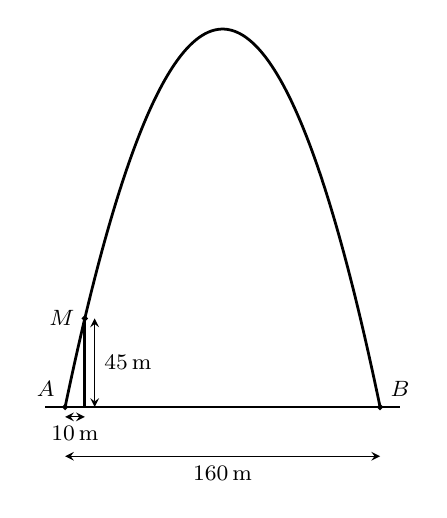
\begin{tikzpicture}[scale=0.25,line width=1pt,>=stealth,x=1mm,y=1mm]
          \draw (-10,0)--(0,0) node[above left] {\footnotesize $A$} -- (160,0) node[above right]{\footnotesize $B$}--(170,0) (10,45) node[left]{\footnotesize $M$};
          \draw(10,0)--(10,45);
          \draw[<->,thin](15,0)--(15,45) node[midway,right]{\footnotesize $45\,\mathrm{m}$};
          \draw[<->,thin] (0,-5)--(10,-5) node[midway,below]{\footnotesize $10\,\mathrm{m}$};
          \draw[<->,thin]  (0,-25)--(160,-25)node[midway,below]{\footnotesize $160\,\mathrm{m}$};
          \draw[fill=black](0,0) circle (2pt) (10,45) circle (2pt) (160,0) circle (2pt);
          \usepgflibrary{fpu}
          \draw[smooth,samples=100,domain=0:160,/pgf/fpu,/pgf/fpu/output format=fixed] plot(\x,{-0.03*(\x)^2+4.8*(\x)});
      \end{tikzpicture}
  }
  \loigiai{
      \immini{Đặt hệ trục toạ độ với $Axy$ như hình vẽ.\\
          Xét parabol $(P):\,y=ax^2+bx+c$.\\
          $M\in(P)\Leftrightarrow100a+10b+c=45$\\
          $A\in(P)\Leftrightarrow c=0$. $B\in(P)\Leftrightarrow160^2a+160b+c=0$.\\
          Giải hệ được $y=-0,03x^2+4,8x$.\\
          $\Rightarrow$ Chiều cao cổng là $y(80)=192\,\mathrm{m}$.
      }
      {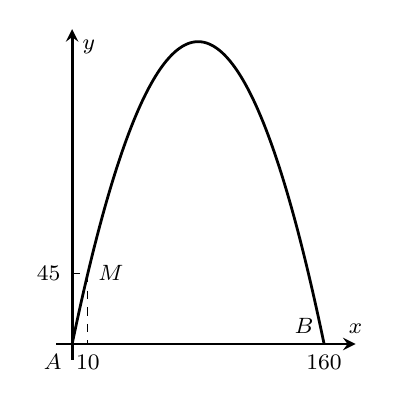
\begin{tikzpicture}[scale=0.2,line width=1pt,>=stealth,x=1mm,y=1mm]
              \draw (0,0) node[below left] {\footnotesize $A$} (10,45) node[right]{\footnotesize $M$} (160,0) node[above left]{\footnotesize $B$};
              \draw[->] (-10,0) -- (180,0) node [above] {\footnotesize$x$};
              \draw[->] (0,-10) -- (0,200) node [below right] {\footnotesize$y$};
              \foreach \x/\xtext in {10/10,160/160}
              \draw[shift={(\x,0)}] (0pt,2pt)--(0pt,-2pt) node[below] {\footnotesize $\xtext$};
              \foreach \y/\ytext in {45/45}
              \draw[shift={(0,\y)}] (2pt,0pt)--(-2pt,0pt) node[left] {\footnotesize $\ytext$};
              \draw[dashed,thin] (0,45)--(10,45)--(10,0);
              \usepgflibrary{fpu}
              \draw[smooth,samples=100,domain=0:160,/pgf/fpu,/pgf/fpu/output format=fixed] plot(\x,{-0.03*(\x)^2+4.8*(\x)});
          \end{tikzpicture}
      }
  }

\end{ex}